\documentclass[a4paper]{article}
\usepackage{geometry}
\usepackage{graphicx}
\usepackage{natbib}
\usepackage{amsmath}
\usepackage{amssymb}
\usepackage{amsthm}
\usepackage{paralist}
\usepackage{epstopdf}
\usepackage{tabularx}
\usepackage{longtable}
\usepackage{multirow}
\usepackage{multicol}
\usepackage[hidelinks]{hyperref}
\usepackage{fancyvrb}
\usepackage{algorithm}
\usepackage{algorithmic}
\usepackage{float}
\usepackage{paralist}
\usepackage[svgname]{xcolor}
\usepackage{enumerate}
\usepackage{array}
\usepackage{times}
\usepackage{url}
\usepackage{fancyhdr}
\usepackage{comment}
\usepackage{environ}
\usepackage{times}
\usepackage{textcomp}
\usepackage{caption}


\urlstyle{rm}

\setlength\parindent{0pt} % Removes all indentation from paragraphs
\theoremstyle{definition}
\newtheorem{definition}{Definition}[]
\newtheorem{conjecture}{Conjecture}[]
\newtheorem{example}{Example}[]
\newtheorem{theorem}{Theorem}[]
\newtheorem{lemma}{Lemma}
\newtheorem{proposition}{Proposition}
\newtheorem{corollary}{Corollary}

\floatname{algorithm}{Procedure}
\renewcommand{\algorithmicrequire}{\textbf{Input:}}
\renewcommand{\algorithmicensure}{\textbf{Output:}}
\newcommand{\abs}[1]{\lvert#1\rvert}
\newcommand{\norm}[1]{\lVert#1\rVert}
\newcommand{\RR}{\mathbb{R}}
\newcommand{\CC}{\mathbb{C}}
\newcommand{\Nat}{\mathbb{N}}
\newcommand{\br}[1]{\{#1\}}
\DeclareMathOperator*{\argmin}{arg\,min}
\DeclareMathOperator*{\argmax}{arg\,max}
\renewcommand{\qedsymbol}{$\blacksquare$}

\definecolor{dkgreen}{rgb}{0,0.6,0}
\definecolor{gray}{rgb}{0.5,0.5,0.5}
\definecolor{mauve}{rgb}{0.58,0,0.82}

\newcommand{\Var}{\mathrm{Var}}
\newcommand{\Cov}{\mathrm{Cov}}

\newcommand{\vc}[1]{\boldsymbol{#1}}
\newcommand{\xv}{\vc{x}}
\newcommand{\Sigmav}{\vc{\Sigma}}
\newcommand{\alphav}{\vc{\alpha}}
\newcommand{\muv}{\vc{\mu}}

\newcommand{\red}[1]{\textcolor{red}{#1}}

\def\x{\mathbf x}
\def\y{\mathbf y}
\def\w{\mathbf w}
\def\v{\mathbf v}
\def\E{\mathbb E}
\def\V{\mathbb V}

% TO SHOW SOLUTIONS, include following (else comment out):
\newenvironment{soln}{
	\leavevmode\color{blue}\ignorespaces
}{}


\hypersetup{
	%    colorlinks,
	linkcolor={red!50!black},
	citecolor={blue!50!black},
	urlcolor={blue!80!black}
}

\geometry{
	top=1in,            % <-- you want to adjust this
	inner=1in,
	outer=1in,
	bottom=1in,
	headheight=3em,       % <-- and this
	headsep=2em,          % <-- and this
	footskip=3em,
}


\pagestyle{fancyplain}
\lhead{\fancyplain{}{Homework 1}}
\rhead{\fancyplain{}{CS 760 Machine Learning}}
\cfoot{\thepage}

\title{\textsc{Homework 1}} % Title

%%% NOTE:  Replace 'NAME HERE' etc., and delete any "\red{}" wrappers (so it won't show up as red)

\author{
	Harry Zhang\\
	9081347016\\
} 

\date{}

\begin{document}
	
	\maketitle 
	
	
	\textbf{Instructions:} 
	This is a background self-test on the type of math we will encounter in class. If you find many questions intimidating, we suggest you drop 760 and take it again in the future when you are more prepared.
	
	Use this latex file as a template to develop your homework.
	Submit your homework on time as a single pdf file to Canvas.
	There is no need to submit the latex source or any code.
	Please check Piazza for updates about the homework.
	
	
	\section{Vectors and Matrices [6 pts]}
	Consider the matrix $X$ and the vectors $\mathbf{y}$ and $\textbf{z}$ below:
	$$
	X = \begin{pmatrix}
		3 & 2 \\ -7 & -5 \\
	\end{pmatrix}
	\qquad \mathbf{y} = \begin{pmatrix}
		2 \\ 1
	\end{pmatrix} \qquad \mathbf{z} = \begin{pmatrix}
		1 \\ -1
	\end{pmatrix}
	$$
	\begin{enumerate}
		\item 	Compute $\mathbf{y}^{T} X \mathbf{z}$\\
			    \begin{soln} 
						\begin{align*}
			    		\mathbf{y}^{T} X \mathbf{z} &= \begin{pmatrix}
			    			2 & 1
			    		\end{pmatrix} \begin{pmatrix}
			    			3 & 2 \\ -7 & -5 \\
			    		\end{pmatrix} \begin{pmatrix}
			    			1 \\ -2
			    		\end{pmatrix} \\
			    		&= \begin{pmatrix}
			    			2 & 1
			    		\end{pmatrix} \begin{pmatrix}
			    			1 \\ -2
			    		\end{pmatrix} \\
			    		&= 2 - 2 \\
			    		&= 0
			    	\end{align*}
				\end{soln}
		\item 	Is $X$ invertible? If so, give the inverse, and if no, explain why not.\\
		        \begin{soln}  
				$det(X) = 3 (-5) - (-2)7 = -1 <0$ \\
				$X$ is invertible because the determinant of $X$ is not zero.
				\end{soln}
	\end{enumerate}
	
	
	\section{Calculus [3 pts]}
	\begin{enumerate}
		\item If $y = e^{-x} + \arctan(z)x^{6/z} - \ln\cfrac{x}{x+1}$, what is the partial derivative of $y$ with respect to $x$?\\
		\begin{soln}\\  
		$\frac{dy}{dx} = -e^{-x} + \frac{6\cdot \arctan(z)}{z} \cdot x^{\frac{6-z}{z}}+\frac{1}{x(x+1)}$ 
		\end{soln}
	\end{enumerate}
	
	
	
	
	\section{Probability and Statistics [10 pts]}
	Consider a sequence of data $S = (1, 1, 1, 0, 1)$ created by flipping a coin $x$ five times, where 0 denotes that the coin turned up heads and 1 denotes that it turned up tails.
	\begin{enumerate}
		\item 	(2.5 pts) What is the probability of observing this data, assuming it was generated by flipping a biased coin with $p(x=1) = 0.6$?
		
		\begin{soln}
		\\
		$P(S) = P(x=1) \cdot P(x=1) \cdot P(x=1) \cdot P(x=1) \cdot P(x=0) = 0.6^4 \cdot 0.4 = 0.05184$
		\end{soln}
		
		\item 	(2.5 pts) Note that the probability of this data sample could be greater if the value of $p(x = 1)$ was not $0.6$, but instead some other value. What is the value that maximizes the probability of $S$? Please justify your answer.\\
		\begin{soln}\\
		Assume: $P(x=1) = p \Rightarrow P(S) = p^4 \cdot (1-p) = p^4 - p^5$\\
		when $p \in (0,1)$, maximum exists if: $\frac{dP(S)}{dp} = 4p^3 - 5p^4 = 0 \Rightarrow p^* = \frac{4}{5}$\\
		When $p = \frac{4}{5}$, $P(S)$ reaches maximum.
		\end{soln}
		
		\item 	(5 pts) Consider the following joint probability table where both $A$ and $B$ are binary random variables: 
		\begin{table}[htb]
			\centering
			\begin{tabular}{ccc}\hline
				A & B & $P(A, B)$  \\\hline
				0 & 0 & 0.3 \\
				0 & 1 & 0.1 \\
				1 & 0 & 0.1 \\
				1 & 1 & 0.5 \\\hline
			\end{tabular}
		\end{table}
		\begin{enumerate}
			\item 	What is $P(A = 0 | B = 1)$?\\
			 \begin{soln}  See table: $P(A=0 | B=1) =\frac{P(\text{while B is 1, A is 0})}{P(\text{B is 1})}= \frac{1}{6}$ \end{soln}
			 
			\item 	What is $P(A = 1 \vee B = 1 )$?\\
		    \begin{soln}
				$P(A=0 \vee B=1) = P(A=1,B=0) + P(A=1,B=1) + P(A=0,B=1) = 0.7$
			\end{soln}
		\end{enumerate}
	\end{enumerate}
	
	
	\section{Big-O Notation [6 pts]}
	For each pair $(f, g)$ of functions below, list which of the following
	are true: $f(n) = O(g(n))$, $g(n) = O(f(n))$, both, or
	neither. Briefly justify your answers.
	\begin{enumerate}
		\item 	$f(n) = \ln(n)$, $g(n) = \log_{2}(n)$.\\
		\begin{soln}\\
		$f(n) = \ln(n) = \frac{\log_{2}(n)}{\log_{2}(e)} = \frac{1}{\log_{2}(e)} \cdot \log_{2}(n) = \frac{1}{\log_{2}(e)} \cdot g(n)$ \\
		$\frac{f(n)}{g(n)} = \ln(2) = O(1) \Rightarrow \frac{f(n)}{g(n)} \rightarrow c$\\
		$\Rightarrow f(n) = O(g(n))$ and $g(n) = O(f(n))$
		\end{soln}
		
		\item 	$f(n) =  \log_{2}\log_{2}(n)$, $g(n) = \log_{2}(n)$.\\
		\begin{soln}\\
		$f(n) = log_2(log_2(n)) = log_2(g(n))$ || $f(n)$ takes $log_2$ of $g(n)$, which means for larger $n$, $g(n)$ both be larger and grows faster than $f(n)$\\
		$\Rightarrow f(n) = O(g(n))$ and $g(n) \neq O(f(n))$
		\end{soln}
		
		\item 	$f(n) = n!$, $g(n) = 2^n$.\\
		\begin{soln}\\
		The growth rate of $f(n)$ is greater than $g(n)$ when $n$ is large \\
		$\Rightarrow g(n) = O(f(n)) $ since $f(n)$ provides upper bounds for $g(n)$ for large $n$; and hence  $f(n) \neq O(g(n))$ \end{soln}
	\end{enumerate}
	
	
	
	
	
	\section{Probability and Random Variables }
	\subsection{Probability [12.5 pts]}
	State true or false. Here $\Omega$ denotes the sample space and $A^c$ denotes the complement of the event $A$.
	\begin{enumerate}
		\item For any $A, B \subseteq \Omega$, $P(A|B)P(A) = P(B|A)P(B)$.\\
		\begin{soln}\\
			It is a False statement. \\
		Known that: $P(A \cap B) = P(A|B) P(B) = P(B|A) P(A)$ \\
		However, we want to prove: $P(A|B)P(A) = P(B|A)P(B)$, which isn't true because $P(A|B) \neq P(B|A)$ in general.\\
		\end{soln}
		
		\item For any $A, B \subseteq \Omega$, $P(A \cup B) = P(A) + P(B) - P(B \cap A)$.\\         
		\begin{soln}\\
			It is a True statement. \\
		$P(A \cup B) = P(A) + P(B) - P(A \cap B)$\\
		Which could be interpreted by definition: probability of $A$ or $B$ is the sum of probability of $A$ and $B$ minus the probability of $A$ and $B$ both happen ($A$ and $B$ both happen is the "intersection" part).
		\end{soln}
		
		\item For any $A, B, C \subseteq \Omega$ such that $P(B \cup C) > 0$,
		$\frac{P(A \cup B \cup C)}{P(B \cup C)} \geq P(A | B \cup C) P(B)$.\\ 
		\begin{soln}\\
		It is a True statement. \\
		$LHS = \frac{P(A \cup B \cup C)}{P(B \cup C)}, \;\;\; RHS = P(A|B \cup C) P(B) =\frac{P(A \cap (B \cup C)) P(B)}{P(B \cup C)}\;\;$ since denominators are the same for RHS and LHS, we only need to compare the numerators\\
		Assume: $B \cup C = D$\\
		$P(A \cap (B \cup C)) = P(A \cap D) \leq P(A)$\\
		$P(A \cup (B \cup C)) = P(A \cup D) \geq P(A)$\\
		$\Rightarrow P(A \cap D) \leq P(A \cup D) \Rightarrow P(A \cap (B \cup C)) \leq P(A \cup (B \cup C))$\\
		since $0 \leq P(B) \leq 1 \Rightarrow P(A \cup (B \cup C)) \geq P(A \cap (B \cup C)) P(B)\Rightarrow LHS \geq RHS$\\
		\end{soln}
		
		\item For any $A, B\subseteq\Omega$ such that $P(B) > 0, P(A^c) > 0$,
		$P(B|A^C) + P(B|A) = 1$.\\ 
		\begin{soln}\\
		It is a False statement. \\
		By total probability law: $P(B) = P(A^c)P(B|A^c) + P(A)P(B|A) $\\
		We can find a counterexample while $P(B) > 0, P(A^c) > 0$ and $P(A) > 0$ which will make $P(B|A^C) + P(B|A) \neq 1$\\
		\end{soln}
		
		\item If $A$ and $B$ are independent events, then $A^{c}$ and $B^{c}$ are independent.\\
		\begin{soln}\\
			It is a True statement. \\
		$A$ and $b$ are independent events $\Rightarrow P(A \cap B) = P(A)P(B)$\\
		$P(A^c \cap B^c) = P((A \cup B)^c) = 1 - P(A \cup B) = 1 - (P(A)+P(B)- P(A \cap B)) = 1 - P(A) - P(B) + P(A)P(B) = (1-P(A))(1-P(B)) = P(A^c)P(B^c)$\\
		Therefore, $A^c$ and $B^c$ are independent events.
		\end{soln}
		
	\end{enumerate}
	
	\subsection{Discrete and Continuous Distributions [12.5 pts]}
	Match the distribution name to its probability density / mass
	function. Below, $|\xv| = k$.
	\begin{enumerate}[(a)]
		\begin{minipage}{0.3\linewidth}
			\item Gamma \begin{soln}  (j) \end{soln}
			\item Multinomial  \begin{soln}  (i) \end{soln}
			\item Laplace \begin{soln}  (h) \end{soln}
			\item Poisson \begin{soln}  (l) \end{soln}
			\item Dirichlet  \begin{soln}  (k) \end{soln}
			
		\end{minipage}
		\begin{minipage}{0.5\linewidth}
			\item $f(\xv; \Sigmav, \muv) = \frac{1}{\sqrt{(2\pi)^k \mathrm{det}(\Sigmav) }} \exp\left( -\frac{1}{2}
			(\xv - \muv)^T \Sigmav^{-1} (\xv - \muv)  \right)$
			\item $f(x; n, \alpha) = \binom{n}{x} \alpha^x (1 - \alpha)^{n-x}$
			for $x \in \{0,\ldots, n\}$; $0$ otherwise
			\item $f(x; b, \mu) = \frac{1}{2b} \exp\left( - \frac{|x - \mu|}{b} \right)$
			\item $f(\xv; n, \alphav) = \frac{n!}{\Pi_{i=1}^k x_i!}
			\Pi_{i=1}^k \alpha_i^{x_i}$ for $x_i \in \{0,\ldots,n\}$ and
			$\sum_{i=1}^k x_i = n$; $0$ otherwise
			\item $f(x; \alpha, \beta) = \frac{\beta^{\alpha}}{\Gamma(\alpha)} x^{\alpha -
				1}e^{-\beta x}$ for $x \in (0,+\infty)$; $0$ otherwise
			\item $f(\xv; \alphav) = \frac{\Gamma(\sum_{i=1}^k
				\alpha_i)}{\prod_{i=1}^k \Gamma(\alpha_i)} \prod_{i=1}^{k}
			x_i^{\alpha_i - 1}$ for $x_i \in (0,1)$ and $\sum_{i=1}^k x_i =
			1$; 0 otherwise
			\item $f(x; \lambda) = \lambda^x \frac{e^{-\lambda}}{x!}$ for all
			$x \in Z^+$; $0$ otherwise
		\end{minipage}
	\end{enumerate}
	
	\subsection{Mean and Variance [10 pts]}
	\begin{enumerate}
		\item Consider a random variable which follows a Binomial
		distribution: $X \sim \text{Binomial}(n, p)$.
		\begin{enumerate}
			\item What is the mean of the random variable?\\
			\begin{soln}\\
			$\mathbb{E}(x) = np$
			\end{soln}
			\item What is the variance of the random variable?\\
			\begin{soln}  \\
				$Var(x) = np(1-p)$
			\end{soln}
		\end{enumerate}
		
		\item Let $X$ be a random variable and
		$\mathbb{E}[X] = 1, \Var(X) = 1$. Compute the following values:
		\begin{enumerate}
			\item $\mathbb{E}[5X]$\\
			\begin{soln}\\
			$\mathbb{E}(5X) = 5$
			\end{soln}
			\item $\Var(5X)$\\
			\begin{soln}\\
			$Var(5X) = 25$
			\end{soln}
			\item $\Var(X+5)$\\
			\begin{soln}\\
			$Var(X+5) = Var(X) = 1$
			\end{soln}
		\end{enumerate}
	\end{enumerate}
	
	%\clearpage
	
	\subsection{Mutual and Conditional Independence [12 pts]}
	\begin{enumerate}
		\item (3 pts) If $X$ and $Y$ are independent random variables, show that
		$\mathbb{E}[XY] = \mathbb{E}[X]\mathbb{E}[Y]$.
		
		\begin{soln}\\
		By definition: $\mathbb{E}[XY] = \sum_x \sum_y x y \cdot P(X=x,Y=y) = \sum_x \sum_y x y \cdot P(X=x) \cdot P(Y=y)= \sum_x \cdot P(X=x) \sum_y y \cdot P(Y=y)  = \mathbb{E}[X]\mathbb{E}[Y]$
		\end{soln}
		
		\item (3 pts) If $X$ and $Y$ are independent random variables, show that
		$\Var(X+Y) = \Var(X) + \Var(Y)$. \\
		Hint: $\Var(X+Y) = \Var(X) + 2\Cov(X, Y) + \Var(Y)$
		
		\begin{soln}\\
			$\Var(X+Y) = \Var(X) + 2\Cov(X, Y) + \Var(Y)$ \\
			for independent variables: $\mathbb{E}(XY) = \mathbb{E}(X) \mathbb{E}(Y) \Rightarrow \Var(X+Y) = \Var(X) + 2(\mathbb{E}(XY) - \mathbb{E}(X)\mathbb{E}(Y)) + \Var(Y) = \Var(X) + \Var(Y)$   \\
		\end{soln}
		
		\item (6 pts) If we roll two dice that behave independently of each
		other, will the result of the first die tell us something about the
		result of the second die? 
		
		\begin{soln}\\
		No, because definition of independent events is the result of them doesn't depend on each others\end{soln}
		
		If, however, the first die's result is a 1,
		and someone tells you about a third event --- that the sum of the two
		results is even --- then given this information is the result of the second die
		independent of the first die? 
		
		\begin{soln}\\
		Yes, in this case, if the sum of the first two dices is even which could be ${2,4,6,8,10,12}$, and I know the first dice's result is 1, then the second dice's result can only be ${1,3,5}$, which means the result of the second dice is dependent on the first dice's result.
		\end{soln}
	\end{enumerate}
	
	\subsection{Central Limit Theorem [3 pts]}
	Prove the following result.
	\begin{enumerate}
		\item Let $X_i\sim\mathcal{N}(0, 1)$ and $\bar{X} = \frac{1}{n}\sum_{i=1}^n X_i$, then the distribution of $\bar{X}$ satisfies 
		$$\sqrt{n}\bar{X}\overset{n\rightarrow\infty}{\longrightarrow}\mathcal{N}(0, 1)$$
		
		\begin{soln}\\
		$\mathbb{E}(\sqrt{n}\bar{X}) = \sqrt{n} \frac{1}{n}\sum_{i=1}^n \mathbb{E}(X_i) = 0$\\ 
		$\Var(\sqrt{n}\bar{X}) = \sqrt{n}^2 \frac{1}{n^2}\sum_{i=1}^n \Var(X_i) = \frac{1}{n} n = 1 \Rightarrow \sigma(\bar{X}) = 1$\\
		As $n$ becomes large, $\sqrt{n}\bar{X}$ will converge to $\mathcal{N}(0, 1)$ according to the central limit theorem.
		\end{soln}
		
	\end{enumerate}
	
	
	
	\section{Linear algebra}
	
	
	\subsection{Norms [5 pts]}
	Draw the regions corresponding to vectors $\mathbf{x}\in\RR^2$ with the following norms:
	\begin{enumerate}
		\item 	$||\mathbf{x}||_1\leq 1$ (Recall that $||\mathbf{x}||_1 = \sum_i |x_i|$)

	\begin{soln}
		%Solution figure goes here.\\
	    % add figure filename, and remove % 
	    %    (this can be done by highlighting text and pressing "cmd + /" for sharelatex+mac)
	   \begin{figure}[h!]
	       \centering
	       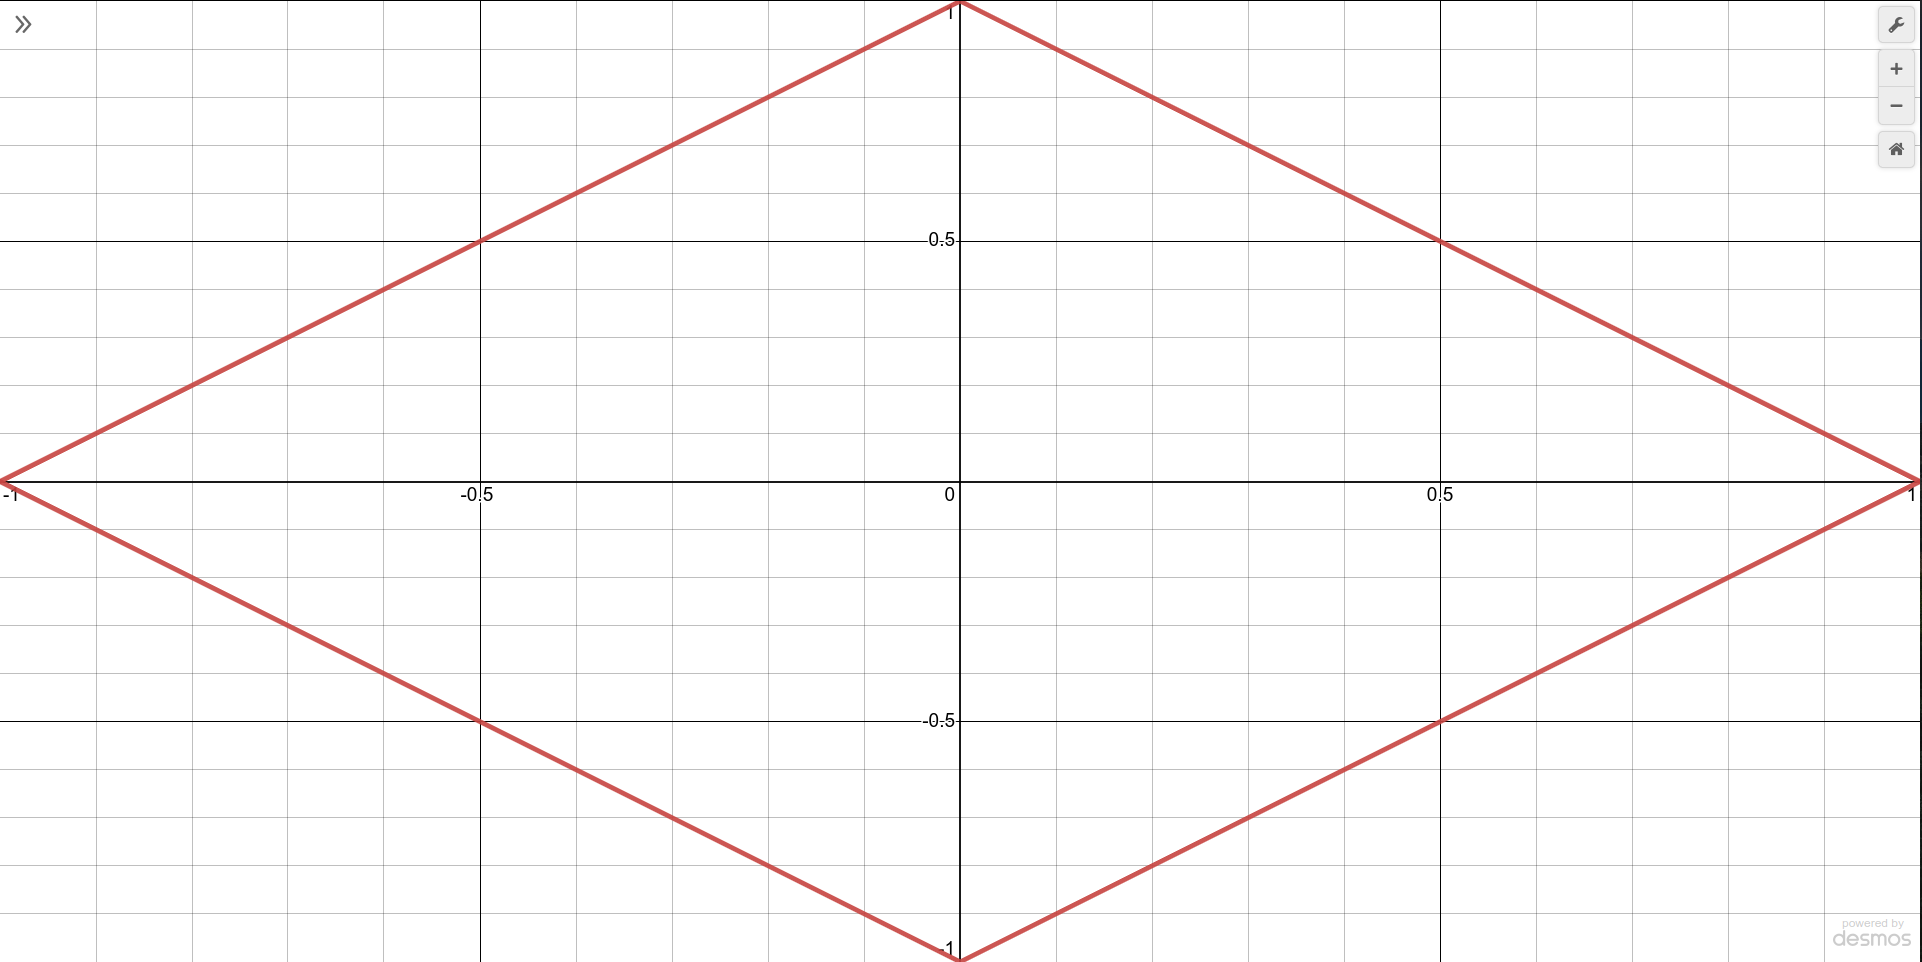
\includegraphics[width=0.4\textwidth]{images/l1.png}  
	               % reference folder/figure.pdf here and adjust width
	       \captionsetup{labelformat=empty}
	       \caption{$||\mathbf{x}||_1\leq 1$}
	       \label{fig:l1}
	   \end{figure}
	\end{soln}
		
		\item 	$||\mathbf{x}||_2 \leq 1$ (Recall that $||\mathbf{x}||_2 =\sqrt{\sum_i x_i^2}$)
			\begin{soln}
			% add figure filename, and remove % 
			%    (this can be done by highlighting text and pressing "cmd + /" for sharelatex+mac)
			\begin{figure}[h!]
			    \centering
			    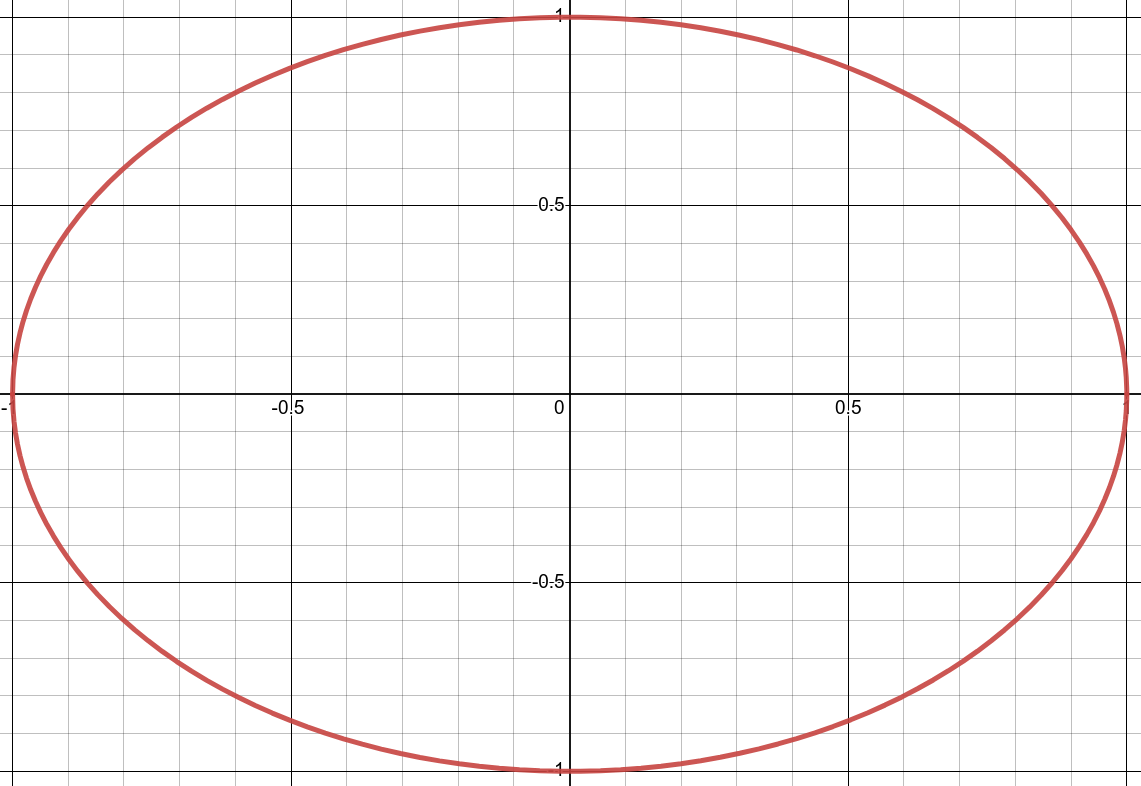
\includegraphics[width=0.4\textwidth]{images/l2.png}  
			            % reference folder/figure.pdf here and adjust width
			    \captionsetup{labelformat=empty}
			    \caption{$||\mathbf{x}||_2 \leq 1$}
			    \label{fig:l2}
			\end{figure}
		\end{soln}
		\item 	$||\mathbf{x}||_\infty \leq 1$ (Recall that $||\mathbf{x}||_\infty = \max_i |x_i|$)
			\begin{soln}
			% add figure filename, and remove % 
			%    (this can be done by highlighting text and pressing "cmd + /" for sharelatex+mac)
			\begin{figure}[h!]
			    \centering
			    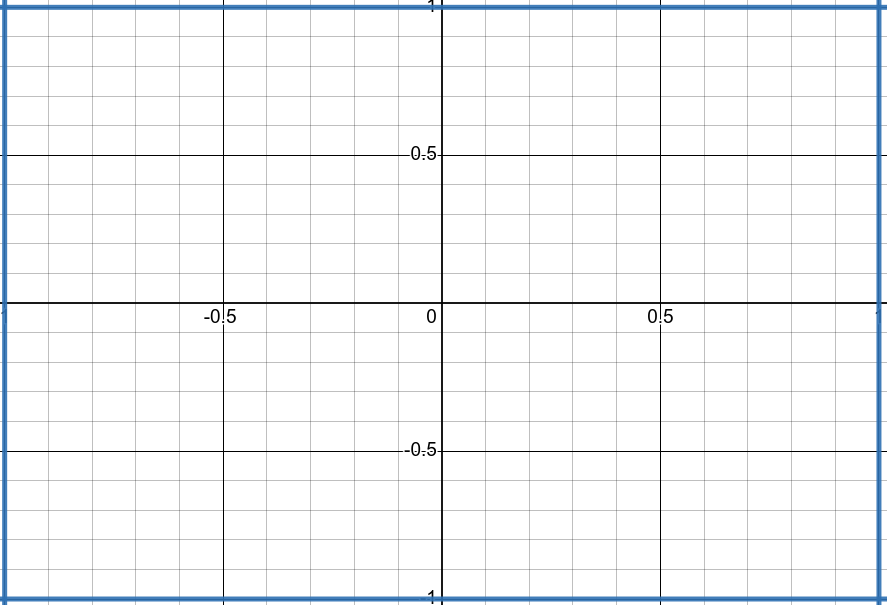
\includegraphics[width=0.4\textwidth]{images/l3.png}  
			            % reference folder/figure.pdf here and adjust width
			    \captionsetup{labelformat=empty}
			    \caption{$||\mathbf{x}||_\infty \leq 1$}
			    \label{fig:l3}
			\end{figure}
		\end{soln}
	\end{enumerate}
	
	For $M = \begin{pmatrix}
		5 & 0 & 0 \\ 0 & 7 & 0 \\ 0 & 0 & 3
		
	\end{pmatrix}$, Calculate the following norms.
	\begin{enumerate}\addtocounter{enumi}{3}
		\item $||M||_{2}$ (L2 norm) \\
		\begin{soln}\\
			$||M||_2 = \sqrt{\lambda_{max}(M^TM)} = \sqrt{\lambda_{max}(M^2)} = \sqrt{\lambda_{max}(\begin{pmatrix}
				25 & 0 & 0 \\ 0 & 49 & 0 \\ 0 & 0 & 9
			\end{pmatrix})} = \sqrt{49} = 7$
		\end{soln}
		
		\item $||M||_{F}$ (Frobenius norm)\\
		\begin{soln}\\
			$||M||_F  = \sqrt{\sum M_{i,j}} = \sqrt{25+49+9} = \sqrt{83}$
		\end{soln}
		
		
	\end{enumerate}
	
	
	
	\subsection{Geometry [10 pts]}
	Prove the following.  Provide all steps.
	\begin{enumerate}
		\item 	The smallest Euclidean distance from the origin to some point $\mathbf{x}$ in the hyperplane $\mathbf{w}^{T}\mathbf{x} + b = 0$ is $\frac{|b|}{||\mathbf{w}||_2}$.  You may assume $\mathbf{w} \neq 0$.\\
		\begin{soln}\\
		The minimum distance from the origin to a point $\mathbf{x}$ is $d = ||proj_\omega \mathbf{(0 - x)}||_2 \;\; s.t. -\mathbf{w}^{T}\mathbf{x} = b  \Rightarrow d = ||\frac{-\mathbf x \cdot \mathbf{\omega}}{\mathbf\omega \cdot \mathbf\omega} \mathbf\omega|| = \frac{|b|}{||\mathbf{\omega}||_2}$.\\
		\end{soln}
		
		\item 	The Euclidean distance between two parallel hyperplane $\mathbf{w}^{T}\mathbf{x} + b_1 = 0$ and $\mathbf{w}^{T}\mathbf{x} + b_2 = 0$ is $\frac{|b_1 - b_2|}{||\mathbf{w}||_2}$ (Hint: you can use the result from the last question to help you prove this one).
		
		\begin{soln}\\
		From last question: we can obtain: $d_1 = \frac{|b_1|}{||\mathbf{w}||_2}$ and $d_2 = \frac{|b_2|}{||\mathbf{w}||_2}$ where $d_1$ and $d_2$ are the distances from hyperplanes to origin.\\
		Assume distance between these two hyperplane is: $d = d_1 - d_2 = \frac{|b_1|}{||\mathbf{w}||_2} - \frac{|b_2|}{||\mathbf{w}||_2} = \frac{|b_1 - b_2|}{||\mathbf{w}||_2}$\\
		\end{soln}
		
	\end{enumerate}
	
	
	
	\section{Programming Skills [10 pts]}
	Sampling from a distribution.  For each question, submit a scatter plot (you will have 2 plots in total).  Make sure the axes for all plots have the same ranges.
	\begin{enumerate}
		\item Make a scatter plot by drawing 100 items from a two dimensional Gaussian $N((1, -1)^{T}, 2I)$, where I is an identity matrix in $\mathbb{R}^{2 \times 2}$.
		
			\begin{soln}
			% Solution figure goes here.\\
			% add figure filename, and remove % 
			%    (this can be done by highlighting text and pressing "cmd + /" for sharelatex+mac)
			\begin{figure}[h!]
			    \centering
			    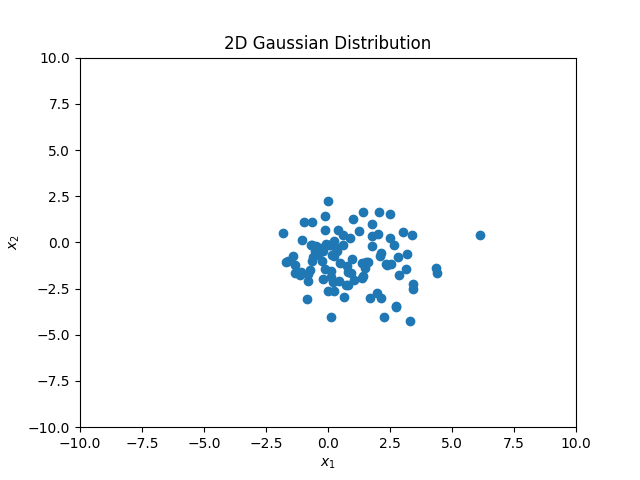
\includegraphics[width=0.25\textwidth]{images/2d_gaussian.png}  
			            % reference folder/figure.pdf here and adjust width
			    \captionsetup{labelformat=empty}
			    \caption{2D Gaussian Distribution}
			    \label{fig:2dgaussian}
			\end{figure}
		\end{soln}
	
		\item Make a scatter plot by drawing 100 items from a mixture distribution 
		$0.3 N\left((5, 0)^{T}, \begin{pmatrix} 1 & 0.25 \\ 0.25 & 1\\ \end{pmatrix}\right)
		+0.7 N\left((-5, 0)^{T}, \begin{pmatrix} 1 & -0.25 \\ -0.25 & 1\\ \end{pmatrix}\right)
		$.
		
		\begin{soln}
		% Solution figure goes here.\\
		% add figure filename, and remove % 
		%    (this can be done by highlighting text and pressing "cmd + /" for sharelatex+mac)
		\begin{figure}[h!]
		    \centering
		    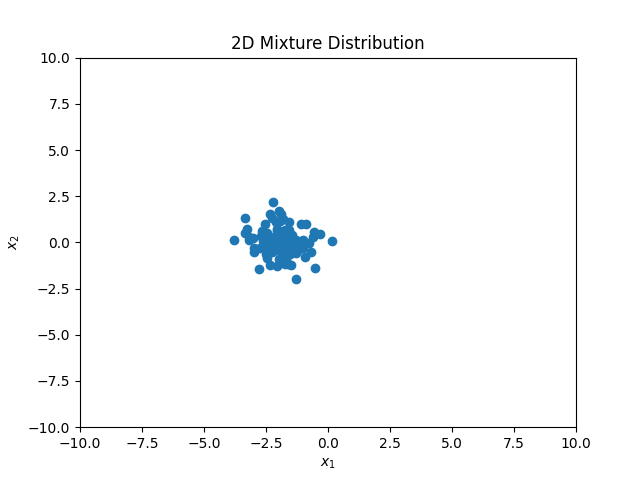
\includegraphics[width=0.25\textwidth]{images/2d_sumdata.png}  
		            % reference folder/figure.pdf here and adjust width
		    \captionsetup{labelformat=empty}
		    \caption{2D Mixture Distribution}
		    \label{fig:mixdist}
		\end{figure}
	\end{soln}
	\end{enumerate}
	
	
	\bibliographystyle{apalike}
	
	
	%----------------------------------------------------------------------------------------
	
	
\end{document}
